\documentclass[numbering=fraction]{beamer}

\usepackage[utf8]{inputenc}
\usepackage[T1]{fontenc}
\usepackage[french]{babel}
\usepackage{blindtext}
\usepackage{tikzsymbols}
\usepackage{graphicx}
\usepackage{wrapfig}
\usepackage{bookman}
\usepackage{subcaption}
\usepackage[export]{adjustbox}


 % possibilité de démos
\usetheme[progressbar=frametitle]{metropolis}

%Define colors
\definecolor{wuppergreen}{RGB}{85, 171, 38}
\definecolor{background}{RGB}{255,255,255}

%Adding logo to title page
\titlegraphic{\raggedleft 
\includegraphics[width=3cm]{UNamur.png}}

%Adjust color theme
\setbeamercolor{frametitle}{bg=wuppergreen}
\setbeamercolor{title separator}{fg=wuppergreen}
\setbeamercolor{footline}{fg=gray}
\setbeamercolor{progress bar}{fg=black}

%Adding footer
\setbeamertemplate{frame footer}{\insertshortauthor~(\insertshortinstitute)}

\graphicspath{ {../Images/}}

%Set parameters for title page
\title{PIMS : Sprint Review 4}
\author[PIMS]{Luis Dierick \and Gaillard Matthys \and Bouncer Yassine \and Fundu Oliver \and Anderson Rosny \and Tom Marchal }
\institute{Université de Namur}
\date{\today}

\begin{document}

\begin{frame}[plain]{}
    \maketitle
\end{frame}

\begin{frame}{Table des matières}
    \tableofcontents
\end{frame}
\section{Rappel des événements de ce qu'il y a été fait}
\begin{frame}{Rappel}
    \begin{itemize}
        \item \textbf{Sprint 1} :
        \begin{itemize}
            \item Enquête de terrain : cellule TICE 
            \item Choix technologiques
        \end{itemize}
        \item \textbf{Sprint 2} : 
        \begin{itemize}
            \item Écriture de mockups et des scénarios en fonction des utilisateurds
        \end{itemize}
        \item \textbf{Sprint 3} :
        \begin{itemize}
            \item Début de la création de l'application
            \item Conception de la base de données.
        \end{itemize}
        \item \textbf{Sprint 4} :
        \begin{itemize}
            \item Création de la partie administration
            \item Gestion des rôles
        \end{itemize}
            
    \end{itemize}
\end{frame}
\section{Ce qui a été fait durant ce sprint}
\subsection{Burndown Chart}
\begin{frame}{Burndown chart}
    \centering
    
    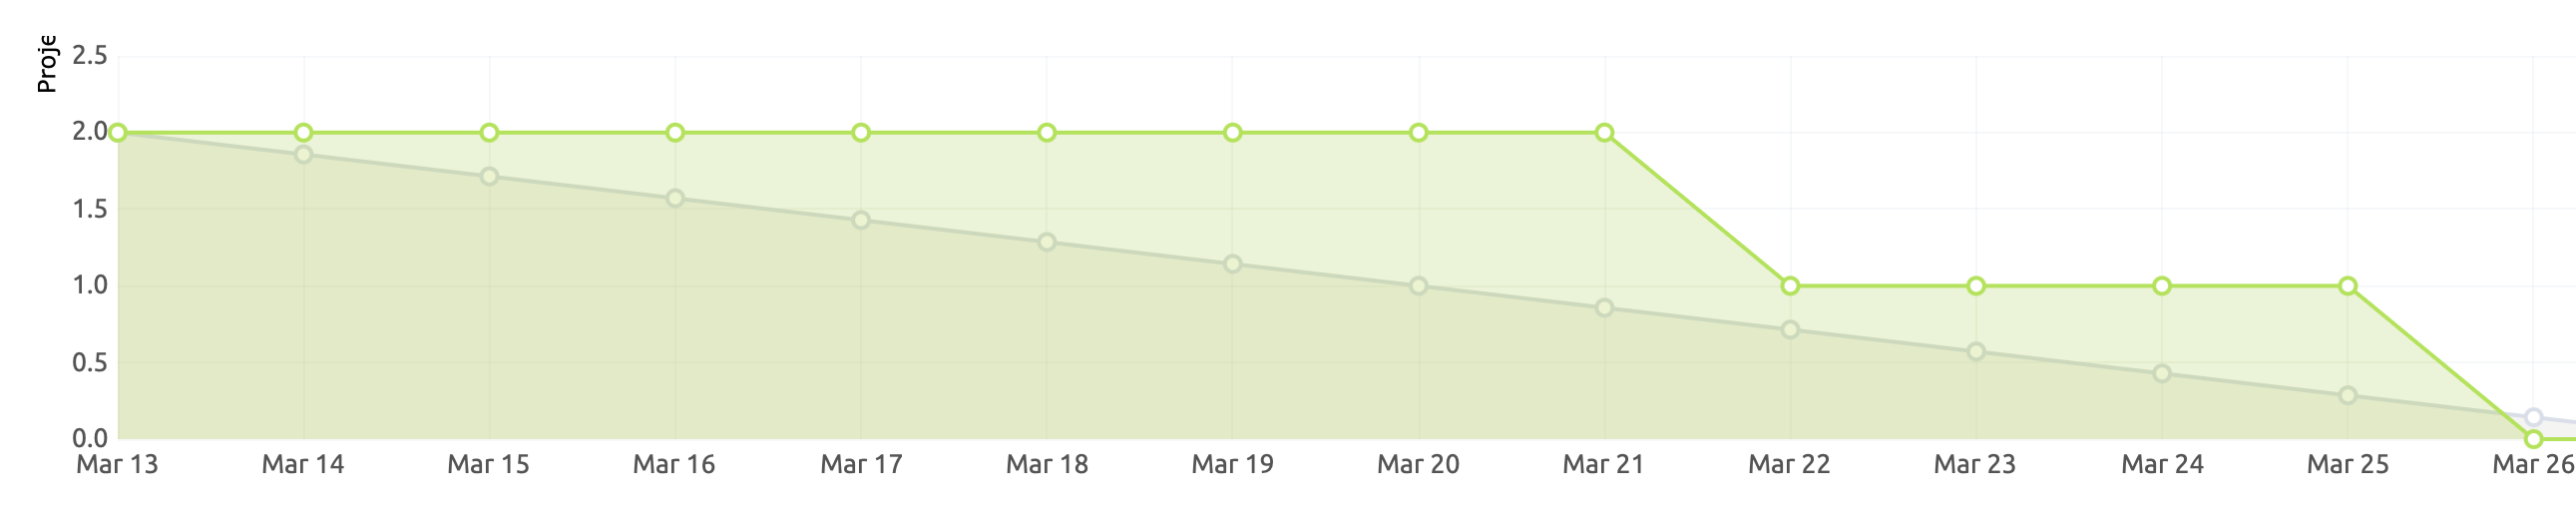
\includegraphics[width=1.1\textwidth]{burndownChart.png} 
\end{frame}

\subsection{Gestion du processus d'inscription}
\begin{frame}{Gestion des cours}
    \begin{columns}
        \begin{column}{0.5\textwidth}
            \begin{enumerate}
                \item Possibilité d'inscription
                \item Possibilité de voir ces cours
            \end{enumerate}
        \end{column}
        \begin{column}{0.5\textwidth}
            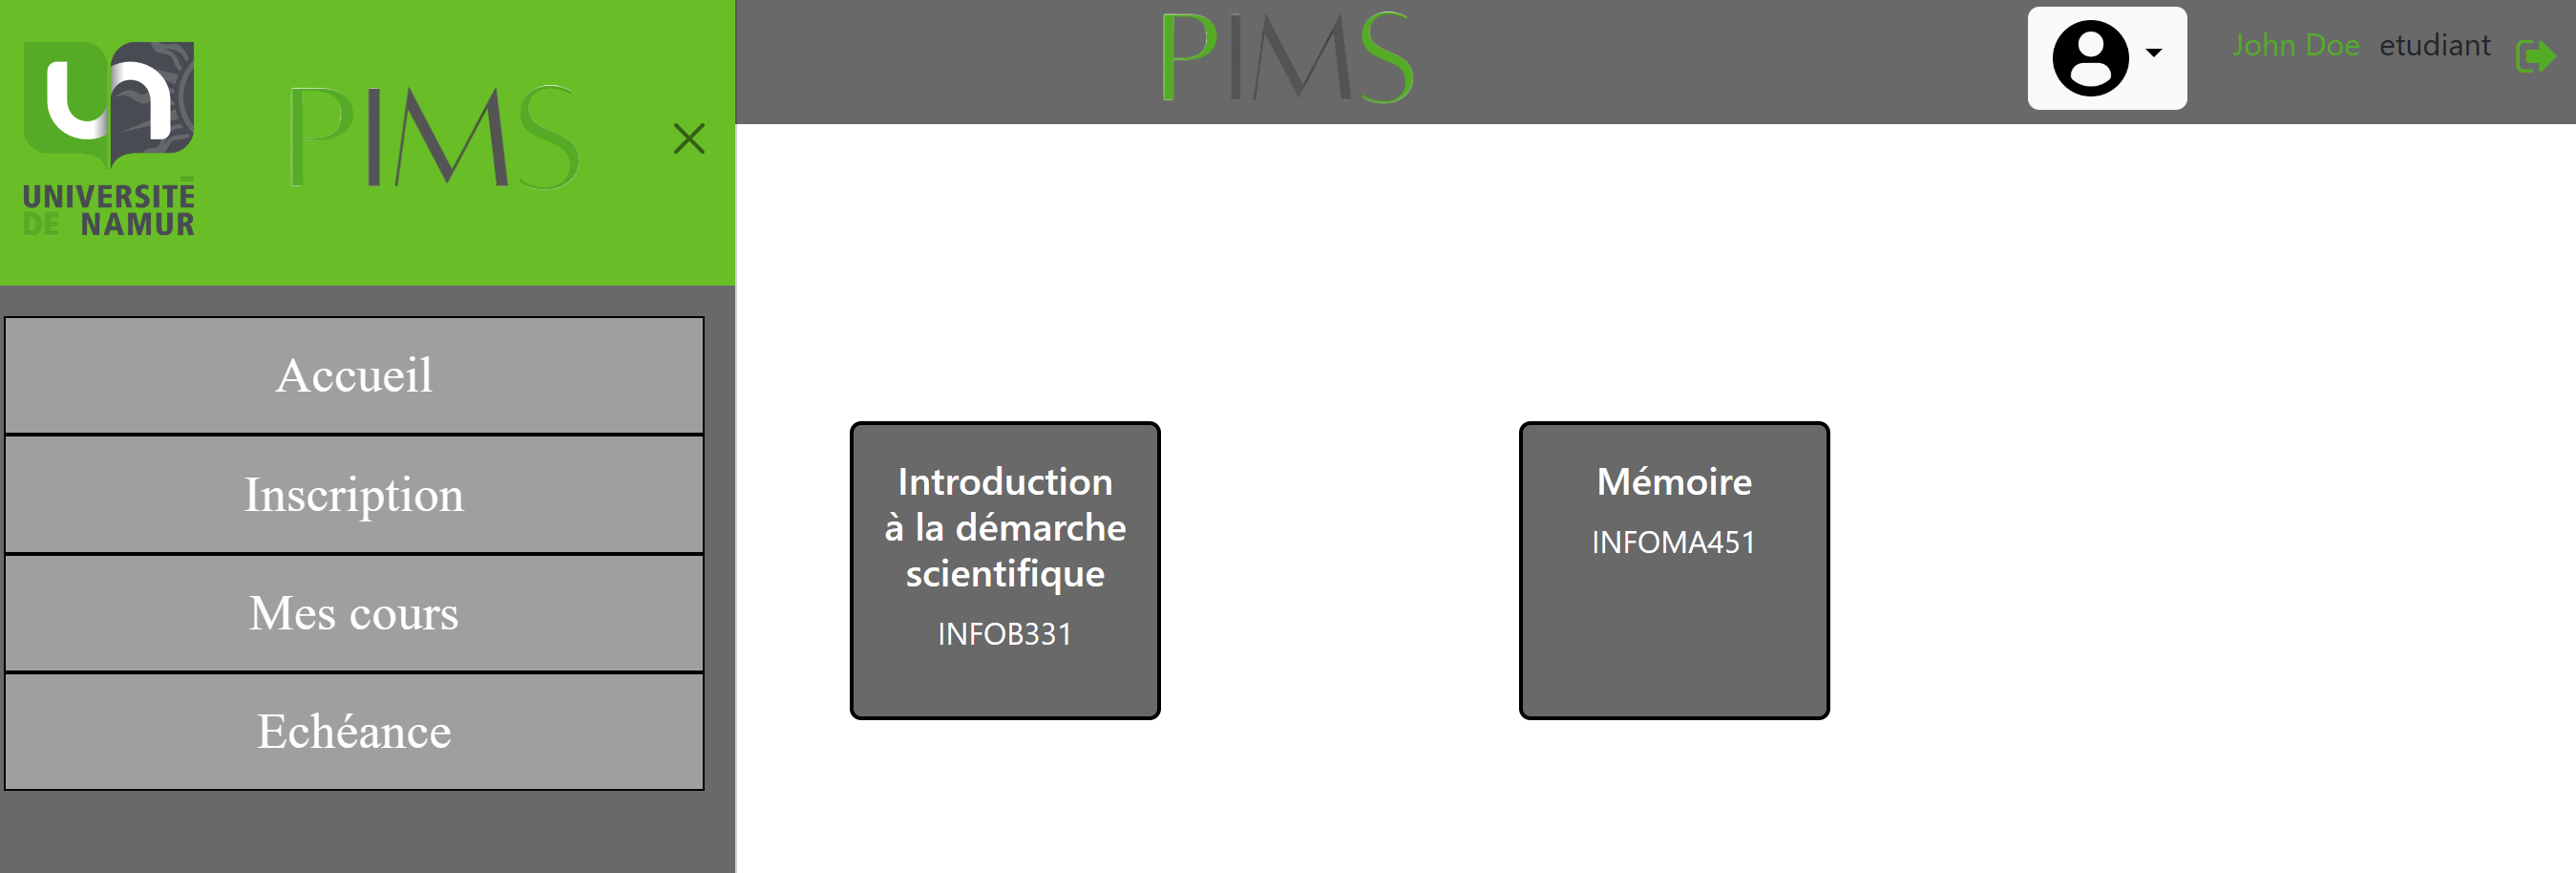
\includegraphics[width=\textwidth]{Gestion cours.png}
        \end{column}
    \end{columns}
\end{frame}
% Yassine modifie me truc
\subsection{Modification graphiques}
\subsection{Modification de la BD}
\begin{frame}{Modification de la BD}
    \begin{enumerate}
        \item Intégration du rôle de superviseur.
        \item Un sujet relié vers un étudiant
        \begin{itemize}
            \item Possibilité d'un sujet par cours.
        \end{itemize}
    \end{enumerate}
\end{frame}
\begin{frame}{Gestion des cours : illustration}
    \centering % Centrer le contenu
\vfill % Remplir l'espace vertical pour centrer verticalement
\textbf{\Large Démonstration} % Texte en gras et en grande taille
\vfill %
    \end{frame}
\section{Echéances prévues}
\begin{frame}{Echéances prévues}
    \begin{enumerate}
        \item Terminer le plus possibles selon l'ordre des priorités les pages web.
        \item Ajout de la desincription  
        \item Mise en ligne du prototype.  
    \end{enumerate}
\end{frame}

\end{document}